\subsubsection{Kosaraju (SCC com Duas DFS)}
O algoritmo de Kosaraju encontra todos os SCCs de um grafo direcionado
realizando duas DFS: a primeira no grafo original para ordenar os vértices por
tempo de término (usando uma pilha), e a segunda no grafo transposto (com as
arestas invertidas) na ordem da pilha. Sua complexidade de tempo é
$\mathcal{O}(V + E)$.

\paragraph{Pseudo-Código: }\mbox{}\\
\begin{algorithm}[H]
    \SetAlgoLined
    \SetKwFunction{Kosaraju}{Kosaraju}
    \SetKwProg{Fn}{Função}{:}{}

    \Fn{\Kosaraju{$adj, V$}}{
        $visitado \gets$ vetor falso de tamanho $V$\;
        $pilha \gets \emptyset$\;

        \For{$i \gets 0$ \Ate $V - 1$}{
            \Se{$\neg visitado[i]$}{
                \text{DFS1($i$, adj, visitado, pilha)}\;
            }
        }

        $adjT \gets$ \text{inverter todas as arestas de } $adj$\;
        $visitado \gets$ limpar visitados\;
        $sccs \gets \emptyset$\;

        \While{$pilha$ não vazia}{
            $u \gets pilha.pop()$\;
            \Se{$\neg visitado[u]$}{
                $componente \gets \emptyset$\;
                \text{DFS2($u$, adjT, visitado, componente)}\;
                $sccs.add(componente)$\;
            }
        }
        \Retorna $sccs$\;
    }
    \caption{Algoritmo de Kosaraju}
\end{algorithm}

Veja o Kosaraju funcionando em duas etapas:\\ \vspace{0.5cm} \noindent
\begin{minipage}[t]{0.31\textwidth}
    \centering
    \textbf{Passo 1: 1ª DFS (Original)}\\
    \vspace{0.2cm}
    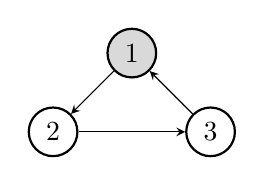
\begin{tikzpicture}[every node/.style={circle, draw, minimum size=0.5cm, thick}, >=stealth]
        \node[fill=gray!30] (1) at (0, 1) {1};
        \node (2) at (-1, 0) {2};
        \node (3) at (1, 0) {3};
        \draw[->] (1) -- (2);
        \draw[->] (2) -- (3);
        \draw[->] (3) -- (1);
    \end{tikzpicture}

    \vspace{0.2cm}
    \footnotesize
    \raggedright
    Executa DFS no grafo original e armazena os nós na pilha por tempo de término.
\end{minipage}%
\hfill
%
\begin{minipage}[t]{0.31\textwidth}
    \centering
    \textbf{Passo 2: Grafo Transposto}\\
    \vspace{0.2cm}
    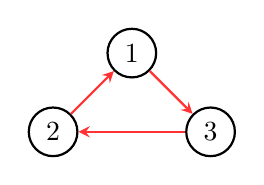
\begin{tikzpicture}[every node/.style={circle, draw, minimum size=0.5cm, thick}, >=stealth]
        \node (1) at (0, 1) {1};
        \node (2) at (-1, 0) {2};
        \node (3) at (1, 0) {3};
        \draw[->, red!80, thick] (2) -- (1);
        \draw[->, red!80, thick] (3) -- (2);
        \draw[->, red!80, thick] (1) -- (3);
    \end{tikzpicture}

    \vspace{0.2cm}
    \footnotesize
    \raggedright
    Inverte todas as arestas do grafo original para formar o grafo transposto ($adjT$).
\end{minipage}%
\hfill
%
\begin{minipage}[t]{0.31\textwidth}
    \centering
    \textbf{Passo 3: 2ª DFS (SCCs)}\\
    \vspace{0.2cm}
    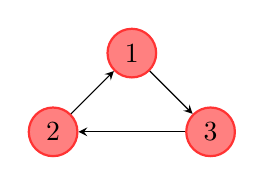
\begin{tikzpicture}[every node/.style={circle, draw, minimum size=0.5cm, thick}, >=stealth]
        \node[fill=red!50, draw=red!80] (1) at (0, 1) {1};
        \node[fill=red!50, draw=red!80] (2) at (-1, 0) {2};
        \node[fill=red!50, draw=red!80] (3) at (1, 0) {3};
        \draw[->] (2) -- (1);
        \draw[->] (3) -- (2);
        \draw[->] (1) -- (3);
    \end{tikzpicture}

    \vspace{0.2cm}
    \footnotesize
    \raggedright
    Executa DFS baseada na pilha. Cada árvore alcançada forma um SCC isolado.
\end{minipage}

\vspace{0.3cm}

\paragraph{Implementação: }\mbox{}\\
\textbf{Python: }
\begin{lstlisting}[language=Python]
def kosaraju(n, adj):
    def dfs1(u):
        visitado[u] = True
        for v in adj[u]:
            if not visitado[v]:
                dfs1(v)
        pilha.append(u)

    def dfs2(u, comp):
        visitado[u] = True
        comp.append(u)
        for v in adjT[u]:
            if not visitado[v]:
                dfs2(v, comp)

    visitado = [False] * n
    pilha = []
    for i in range(n):
        if not visitado[i]:
            dfs1(i)
            
    adjT = [[] for _ in range(n)]
    for u in range(n):
        for v in adj[u]:
            adjT[v].append(u)
            
    visitado = [False] * n
    sccs = []
    while pilha:
        u = pilha.pop()
        if not visitado[u]:
            comp = []
            dfs2(u, comp)
            sccs.append(comp)
    return sccs
\end{lstlisting}

\vspace{0.3cm}
\textbf{C++:}
\begin{lstlisting}[language=C++]
void dfs1(int u, const vector<vector<int>>& adj, vector<bool>& vis, stack<int>& st) {
    vis[u] = true;
    for (int v : adj[u]) if (!vis[v]) dfs1(v, adj, vis, st);
    st.push(u);
}

void dfs2(int u, const vector<vector<int>>& adjT, vector<bool>& vis, vector<int>& comp) {
    vis[u] = true;
    comp.push_back(u);
    for (int v : adjT[u]) if (!vis[v]) dfs2(v, adjT, vis, comp);
}

vector<vector<int>> kosaraju(int n, const vector<vector<int>>& adj) {
    vector<bool> vis(n, false);
    stack<int> st;
    for (int i = 0; i < n; ++i) if (!vis[i]) dfs1(i, adj, vis, st);
    
    vector<vector<int>> adjT(n);
    for (int u = 0; u < n; ++u)
        for (int v : adj[u]) adjT[v].push_back(u);
        
    fill(vis.begin(), vis.end(), false);
    vector<vector<int>> sccs;
    while (!st.empty()) {
        int u = st.top(); st.pop();
        if (!vis[u]) {
            vector<int> comp;
            dfs2(u, adjT, vis, comp);
            sccs.push_back(comp);
        }
    }
    return sccs;
}
\end{lstlisting}
\newpage